% Copyright 2004 by Till Tantau <tantau@users.sourceforge.net>.
%
% In principle, this file can be redistributed and/or modified under
% the terms of the GNU Public License, version 2.
%
% However, this file is supposed to be a template to be modified
% for your own needs. For this reason, if you use this file as a
% template and not specifically distribute it as part of a another
% package/program, I grant the extra permission to freely copy and
% modify this file as you see fit and even to delete this copyright
% notice. 

\documentclass{beamer}

% There are many different themes available for Beamer. A comprehensive
% list with examples is given here:
% http://deic.uab.es/~iblanes/beamer_gallery/index_by_theme.html
% You can uncomment the themes below if you would like to use a different
% one:
%\usetheme{AnnArbor}
%\usetheme{Antibes}
%\usetheme{Bergen}
%\usetheme{Berkeley}
%\usetheme{Berlin}
%\usetheme{Boadilla}
%\usetheme{boxes}
%\usetheme{CambridgeUS}
%\usetheme{Copenhagen}
%\usetheme{Darmstadt}
%\usetheme{default}
%\usetheme{Frankfurt}
%\usetheme{Goettingen}
%\usetheme{Hannover}
%\usetheme{Ilmenau}
%\usetheme{JuanLesPins}
%\usetheme{Luebeck}
\usetheme{Madrid}
%\usetheme{Malmoe}
%\usetheme{Marburg}
%\usetheme{Montpellier}
%\usetheme{PaloAlto}
%\usetheme{Pittsburgh}
%\usetheme{Rochester}
%\usetheme{Singapore}
%\usetheme{Szeged}
%\usetheme{Warsaw}

\usepackage{kotex}
\usepackage{braket}
\usepackage{array}
\usepackage{calc}
\usepackage{datetime}
\usepackage{dsfont}
\usepackage{amsmath}
\usepackage{listings}


\title{Lecture 6 : 적분 / 미분방정식 }

% A subtitle is optional and this may be deleted
\subtitle{Fastcampus Math Camp}

\author{신승우}
% - Give the names in the same order as the appear in the paper.
% - Use the \inst{?} command only if the authors have different
%   affiliation.

% \institute[Universities of Somewhere and Elsewhere] % (optional, but mostly needed)
% {
  % \inst{1}%
  % Department of Computer Science\\
  % University of Somewhere
  % \and
  % \inst{2}%
  % Department of Theoretical Philosophy\\
  % University of Elsewhere}
% - Use the \inst command only if there are several affiliations.
% - Keep it simple, no one is interested in your street address.

% - Either use conference name or its abbreviation.
% - Not really informative to the audience, more for people (including
%   yourself) who are reading the slides online

\subject{Theoretical Computer Science}

% This is only inserted into the PDF information catalog. Can be left
% out. 

% If you have a file called "university-logo-filename.xxx", where xxx
% is a graphic format that can be processed by latex or pdflatex,
% resp., then you can add a logo as follows:

% \pgfdeclareimage[height=0.5cm]{university-logo}{university-logo-filename}
% \logo{\pgfuseimage{university-logo}}

% Delete this, if you do not want the table of contents to pop up at
% the beginning of each subsection:


% \AtBeginSection[]
% {
  % \begin{frame}<beamer>{Outline}
    % \tableofcontents[currentsection,hideallsubsections]
  % \end{frame}
% }

% Let's get started
\begin{document}

\begin{frame}
 \titlepage
\end{frame}


% \begin{frame}{선형변환의 예시 : 확대/축소} 
% 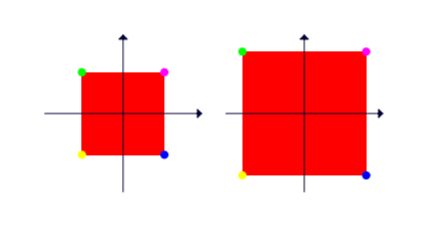
\includegraphics[width=10cm,keepaspectratio]{scale1}
% \end{frame}

% \begin{frame}{Outline}
  % \tableofcontents[hideallsubsections]
  % % You might wish to add the option [pausesections]
% \end{frame}

% Section and subsections will appear in the presentation overview
% and table of contents.

\section{델 연산자} 

\subsection{Gradient} 

\begin{frame}{Vector Field} 
\begin{block}{Vector/Scalar Field} 
Vector Field란 공간 위의 한 점을 벡터 하나로 대응시키는 함수를 말한다. 역으로, Scalar Field란 공간 위의 한 점을 실수 하나로 대응시키는 함수를 말한다. 
\end{block}

Vector Field는 벡터함수로 볼 수 있고, Scalar Field는 스칼라함수로 볼 수 있다. 

\end{frame}

\begin{frame}[allowframebreaks]{Gradient}
스칼라 함수 f에 대해서, 그 함수의 gradient $\nabla f$는 다음과 같이 정의된다. 
\begin{block}{Gradient $\nabla f$} 
$\nabla f = (\frac{\partial f}{\partial x}, \frac{\partial f}{\partial y},\frac{\partial f}{\partial z}) = \frac{\partial f}{\partial x} \hat{x} + \frac{\partial f}{\partial y} \hat{y} + \frac{\partial f}{\partial z} \hat{z}$
\end{block}

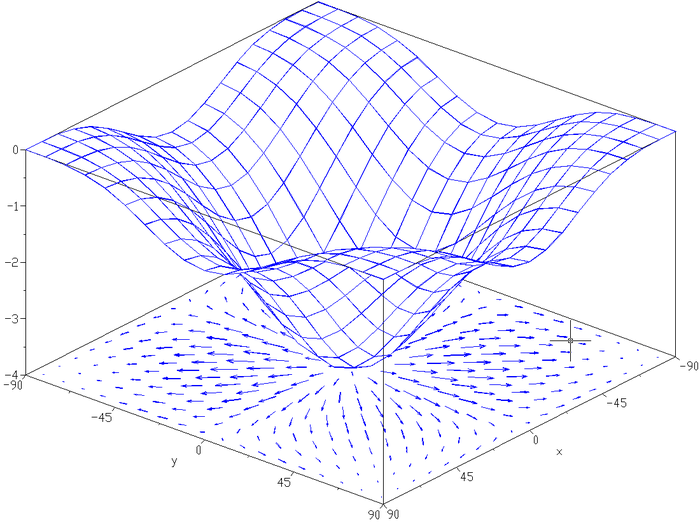
\includegraphics[width=10cm,keepaspectratio]{gradient}

함수의 그래디언트는 함수가 만드는 곡면에서의 기울기를 나타내는 벡터라고 할 수 있다. 그래디언트의 각 항을 살펴보면, $\hat{x}$항은 곧 곡면을 x충에 평행하게 자른 성분의 미분이라고 볼 수 있다. 
\end{frame} 

\begin{frame}{Gradient의 성질} 
스칼라 함수 f,g와 상수 a,b에 대해서 다음이 성립한다. 
\begin{itemize} 
\item $\nabla (af+bg) = a\nabla f + b \nabla g$ 
\item $\nabla fg = f (\nabla g) + (\nabla f) g$
\end{itemize}
\end{frame}

\begin{frame}{Proof for 1)} 

\begin{eqnarray} 
\nabla (af+bg)&=& \sum_i \frac{\partial (af+bg)}{\partial x_i} \\ 
&=& \sum_i [ a\frac{\partial f}{\partial x_i} +  b\frac{\partial g}{\partial x_i} ]\\
&=& a \sum_i \frac{\partial f}{\partial x_i} +  b \sum_i \frac{\partial g}{\partial x_i}  \\ 
&=& a \nabla f + b \nabla g
\end{eqnarray}



\end{frame} 

\begin{frame}{Proof for 2)} 

\begin{eqnarray} 
\nabla fg &=& \sum_i \frac{\partial (fg)}{\partial x_i} \\ 
&=&  \sum_i [f\frac{\partial g}{\partial x_i} +  g\frac{\partial f}{\partial x_i} ]\\
&=&  f \sum_i \frac{\partial g}{\partial x_i} +  g \sum_i \frac{\partial f}{\partial x_i} \\
&=& f \nabla g + g \nabla f
\end{eqnarray}

\end{frame}

\begin{frame}{Gradient의 활용 : Directional Derivative} 

함수 f에 대해서, 특정 방향으로의 미분값을 Directional Derivative라 한다. 함수 f의 벡터 $\vec{a}$로의 Directional Derivative는 다음과 같이 정의된다. 

\begin{equation} 
\nabla_{\vec{a}} f(\vec{x}) = lim_{h \rightarrow 0} \frac{f(\vec{x} + h \vec{a}) - f(\vec{x})}{h}
\end{equation}

이는 그래디언트를 이용하여 다음과 같이 계산될 수 있다. 

\begin{equation} 
\nabla_{\vec{a}}f(\vec{x}) = \nabla f(\vec{x}) \bullet \vec{a}
\end{equation} 

\end{frame}

% proof 

\begin{frame}{Proof} 
위 Directional Derivative의 정의는 아래와 같이 쓰일 수 있다. 

\begin{equation} 
\nabla_{\vec{a}} f(\vec{x}) = lim_{h \rightarrow 0} \frac{f(\vec{x} + h \vec{a}) - f(\vec{x})}{h} = \frac{dF}{dk}
\end{equation}

이 때, $F(k) = f(\vec{x} + h\vec{a})$이고, $k = \vec{x} + h$이다. 이 때, chain rule에 따라서 다음과 같이 정리할 수 있다. 

\begin{eqnarray} 
\frac{dF}{dh} &=& \sum_i \frac{\partial f}{\partial x_i} \frac{dh}{dx_i} \\ 
&=& \sum_i \frac{\partial f}{\partial x_i} \frac{dh}{dx_i} \\
&=& \sum_i \frac{\partial f}{\partial x_i} \vec{a}_i \\
&=& \nabla f \bullet \vec{a} 
\end{eqnarray}

\end{frame}

\begin{frame}{Gradient의 활용 : Multivariate Taylor Expansion} 
스칼라함수 $f(\vec{f})$에 대해서, 다음이 성립한다. 

\begin{equation} 
f(\vec{r} + \vec{\delta}t) = f(\vec{r}) + [\vec{a} \bullet \nabla f(\vec{r}) ] t  + \frac{1}{2!} [\vec{a} \bullet \nabla ]^2 t^2 + ... 
\end{equation} 

즉, 그래디언트는 어떠한 한 점 근방에서 함수를 원하는 찻수의 다항식으로 근사하는 것에 쓰일 수 있다. 

\end{frame}
% proof 

\begin{frame}[allowframebreaks]{Hessian 행렬과 최적화}  
스칼라 함수 f:$\mathds{R}^n \rightarrow \mathds{R}$에 대해서, hessian 행렬 H는 다음과 같이 정의된다. 
\begin{equation} 
H = \left[ \begin{matrix} 
\frac{\partial^2 f}{\partial x_1^2} & \frac{\partial^2 f}{\partial x_1 \partial x_2} & ... & \frac{\partial^2 f}{\partial x_1 \partial x_n} \\ 
\frac{\partial^2 f}{\partial x_2 \partial x_1} & \frac{\partial^2 f}{\partial x_2^2} & ... & \frac{\partial^2 f}{\partial x_2 \partial x_n} \\ 
... & ... & ... & ... \\
\frac{\partial^2 f}{\partial x_n \partial x_1} & \frac{\partial^2 f}{\partial x_n \partial x_2} & ... & \frac{\partial^2 f}{\partial x_n^2} \end{matrix} \right] 
\end{equation} 

이런 Hessian Matrix가 가지는 의미는, 어떤 점 근처에서 원함수 f를 근사하는 2차함수를 만들어낸다는 점이다. 예를 들어서, f가 실수에서 실수로 가는 함수라고 하자. 이 때는 $H = \frac{d^2f}{dx^2}$일 것이다. 즉 이 함수는 테일러급수의 2차항이라고 생각할 수 있다. 이와 비슷하게, 위에서 살펴본 식을 변형하면 n변수 함수에 대해서는 테일러급수의 일반화로 다음이 성립한다. 

\begin{equation} 
f(\vec(x)+\vec{\delta}) \approx f(\vec{x}) + \nabla f(\vec{x})^T \vec{\delta} + \frac{1}{2!} \vec{\delta}^T H(\vec{x}) \vec{\delta}
\end{equation}

이 식을 이용하여 Hessian Matrix를 이용해서 다음을 해 볼 수 있다. 

\begin{itemize} 
\item Second Derivative Test 
\item 최적화
\end{itemize}
에 사용된다. 아래에서 각자의 영역에서 어떻게 사용되는지 살펴보겠다. 

먼저 Second Derivative Test를 살펴보겠다. 먼저, 앞서 수업에서 극값은 다음의 조건을 만족하는 것이 필요조건이라고 하였다. 

\begin{equation} 
\frac{\partial f }{\partial x_i} = 0
\end{equation}

이 때, 위 경우를 만족하면서 극값이 아닌 점을 saddle point라고 한다. 이러한 점을 가려내기 위해서 1변수에서는 2계도함수를 이용하여 판별하였다. 다변수함수의 경우, Hessiam Matrix의  고윳값의 부호를 이용해서 테스트할 수 있다. 즉, 만약 어떤 점 x에서 H의 고윳값이 모두 양수라면 local minimum을 가지고, 모두 음수라면 local maximum을 가지며, 둘 다 아니라면 saddle point가 된다. 예컨대, 다음의 함수를 생각해 보자. 

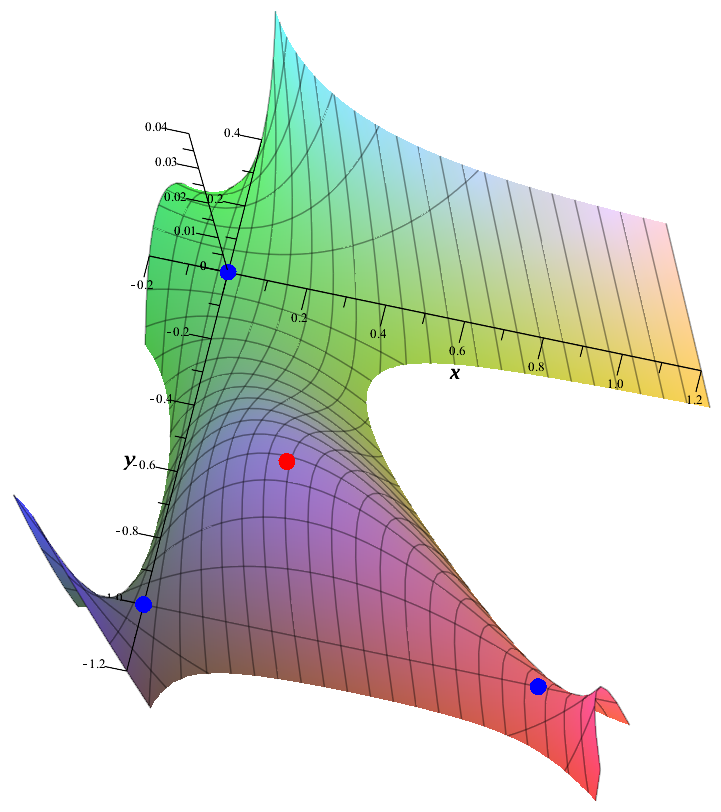
\includegraphics[height=5cm,keepaspectratio]{second}


$f(x,y) = (x+y)(xy+xy^2)$


이 함수는 (0,0), (0,-1), (1,-1), $(\frac{3}{8}, -\frac{3}{4})$에서 $\frac{\partial z}{\partial x} = 0, \frac{\partial z}{\partial y} = 0 $를 만족한다. 이 때, 이 함수의 Hessian 행렬을 구해서 각각의 행렬식을 계산하면 된다. 계산 결과는 다음과 같다. 
\begin{eqnarray}
D(0,0) &=& 0 \\
D(0,-1), D(1, -1) &<& 0\\
D(\frac{3}{8}, -\frac{3}{4}) &>&0
\end{eqnarray}

즉, 두 점에서 saddle point이며 한 점에서는 local maximum을 가지는 것을 알 수 있다. 그리고 (0,0)에서는 이차 미분으로 판별이 불가능하므로, 더 고차 미분을 이용하여 판별하여야 한다. 

두 번째로 최적화에서의 Hessian Matrix를 살펴보겠다. 다시 위 식을 살펴보면, 2차식까지의 근사를 위해서는 Hessian Matrix를 계산하여야 함을 알 수 있다. 즉, n차원의 경우 이를 저장하는 데 $n^2$의 공간과 시간이 필요하다. 이를 해결하기 위해서 일반적으로 Hessian을 직접 계산하는 것이 아니라, 함수의 그래디언트를 미리 계산하여 Hessian을 선형 operator로만 사용하는 것이다. 자세하게는 다음과 같다. 

먼저, 다음 식이 성립한다. 

\begin{equation} 
\nabla f(\vec{x} + \vec{\delta}) \approx \nabla f(\vec{x}) + H(\vec{x})\vec{\delta}
\end{equation} 

따라서 $H \vec{\delta} \approx \nabla f(\vec{x} + \vec{\delta}) - \nabla f(\vec{x}) $이므로, 위 $f(\vec{x} + \vec{\delta})$를 계산할 때 Hessian을 계산하는 것이 아니라 그래디언트를 계산하게 된다. 이에 따라서 계산복잡도는 O(n)이 되어 계산을 효율적으로 수행할 수 있다. 


\end{frame}



\subsection{Divergence} 

\begin{frame}{Divergence의 정의} 
벡터함수 $\vec{F}$에 대해서 그 divergence는 $\nabla$와의 내적으로 정의된다. 즉, 

\begin{block}{Divergence $\nabla \bullet \vec{F}$}
$\nabla \bullet \vec{F} = (\frac{\partial}{\partial x}, \frac{\partial}{\partial y}, \frac{\partial}{\partial z} ) \bullet \vec{F} = \frac{\partial F_x}{\partial x} +  \frac{\partial F_y}{\partial y} + \frac{\partial F_z}{\partial z}$
\end{block}

이다. 
\end{frame}

\begin{frame}{Divergence의 성질} 
상수 a,b와 스칼라함수 f, 벡터함수 $\vec{F}, \vec{G}$에 대해서 다음이 성립한다. 
\begin{itemize} 
\item $\nabla \bullet (a\vec{F} + b\vec{G}) = a \nabla \bullet \vec{F} + b \nabla \bullet \vec{G}$
\item $\nabla \bullet (f \vec{F}) = (\nabla f) \vec{F}  + f \nabla \bullet \vec{F}$
\end{itemize}
\end{frame}

% proof

\subsection{Curl}

\begin{frame}{Curl의 정의} 

벡터함수 $\vec{F}$에 대해서 그 divergence는 $\nabla$와의 외적으로 정의된다. 즉, 
\begin{block}{Divergence $\nabla \bullet \vec{F}$}
$\nabla \bullet \vec{F} = (\frac{\partial}{\partial x}, \frac{\partial}{\partial y}, \frac{\partial}{\partial z} ) \times \vec{F}$\end{block}
\end{frame}

\begin{frame}{Curl의 성질} 
상수 a,b와 스칼라함수 f, 벡터함수 $\vec{F}, \vec{G}$에 대해서 다음이 성립한다. 
\begin{itemize} 
\item $\nabla \times (a\vec{F} + b\vec{G}) = a \nabla \times \vec{F} + b \nabla \times \vec{G}$
\item $\nabla  \times (f \vec{F}) = (\nabla f) \times \vec{F}   + f \nabla \times \vec{F}$
\item $\nabla \times (\vec{F} \times \vec{G}) = \vec{F} (\nabla \bullet \vec{G}) - \vec{G} (\nabla \bullet \vec{F}) + (\vec{G} \bullet \nabla)\vec{F} - (\vec{F} \bullet \nabla) \vec{G}$
\end{itemize}
\end{frame}


\subsection{Operator Identities}


\begin{frame}{Chain Rule}  
\begin{itemize} 
\item $\nabla f(g(\vec{x}) = f^{\prime}g(\vec{x}) \nabla g(x)$ 
\item $\nabla f(\vec{A}(\vec{x})) = \nabla f(\vec{A}(\vec{x})) \nabla \vec{A}$
\item $\nabla \bullet \vec{A}(f(\vec{x})) = \vec{A}^{\prime}(f(\vec{x})) \nabla f$
\item $\nabla \times (\vec{A}(f(\vec{x})) = - \vec{A}^{\prime} (f(\vec{x})) \times \nabla f$
\end{itemize}
\end{frame}

% proof 

% \begin{frame}{Vector Products} 
% \begin{itemize} 
% \item $ \nabla {\vec{A} \bullet \vec{B}) = (\vec{A}
% \end{itemize}
% \end{frame}



\begin{frame}{Second Derivatives} 
\begin{itemize} 
\item Curl of the Gradient : $\nabla \times (\nabla f) = \vec{0}$
\item Divergence of the Curl : $\nabla \bullet (\nabla \times \vec{A}) = 0$ 
\item Divergence of the Gradient : $\nabla(\nabla f) = \nabla^2 f$
\item Curl of the Curl : $\nabla \times (\nabla \times \vec{A}) = \nabla (\nabla \bullet \vec{A}) - \nabla^2\vec{A}$
\end{itemize}
\end{frame}




\section{적분} 

\subsection{적분의 정의} 

\begin{frame}{적분의 정의 : 리만 합} 
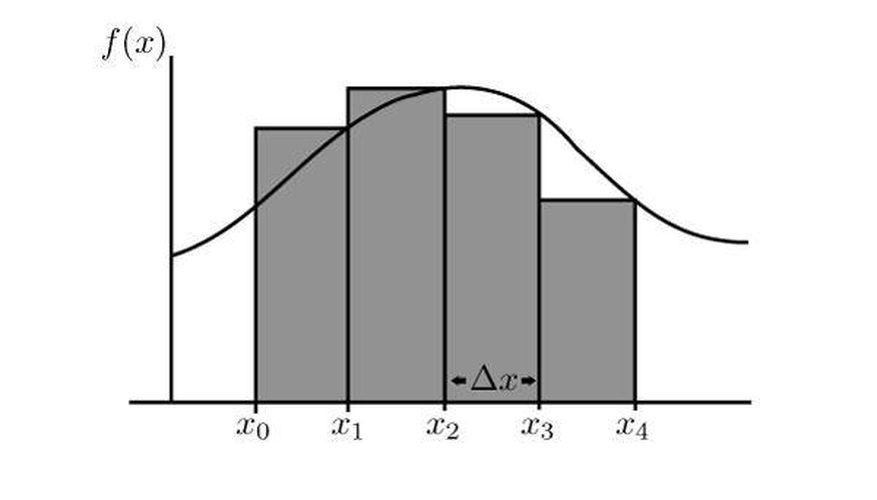
\includegraphics[width=10cm,keepaspectratio]{sum}

어떤 함수 f의 정적분 $\int^{x=b}_{x=a} f(x)dx$ 는 다음과 같이 정의된다. 

\begin{equation} 
S = \int^{x=b}_{x=a} f(x)dx = lim_{n \rightarrow \infty} \sum_i f(a + \frac{(b-a)i}{n}) \delta 
\end{equation} 


\end{frame}

\begin{frame}{적분의 정의 : 미분의 역과정} 
어떤 함수 f의 부정적분 $F=\int f(x)dx$는 다음을 만족하는 함수로 정의된다. 

\begin{equation} 
\frac{dF}{dx} = f
\end{equation}
\end{frame}


\begin{frame}{정적분과 부정적분} 
이 때, 어떤 함수의 a부터 b까지의 정적분 $S = \int^{x=b}_{x=a} f(x)dx$와 함수 f의 부정적분 F(x) 사이에는 다음의 관계가 성립한다. 

\begin{equation} 
F(b) - F(a) = \int^{x=b}_{x=a} f(x)dx
\end{equation} 

이를 미적분학의 기본정리라고 한다. 
\end{frame}

% proof


\subsection{다양한 적분 기법} 


\begin{frame}{부분적분} 

두 함수의 곱의 미분공식을 생각해보자. 

\begin{equation} 
\frac{d(fg)}{dx} = f \frac{dg}{dx} + \frac{df}{dx} g
\end{equation}

이제, 양변을 x로 적분하면 적분의 정의에 의해서 다음과 같다. 

\begin{eqnarray} 
fg &=& \int f \frac{dg}{dx} + \int \frac{df}{dx} g dx \\
\int f \frac{dg}{dx} &=& fg - \int \frac{df}{dx} g dx 
\end{eqnarray} 

위와 같은 방식으로 수행하는 적분을 부분적분이라 한다. 
\end{frame}

\begin{frame}{부분적분의 예시 : $\int e^x sin(x) dx$}
여기서 $f = e^x$, $\frac{dg}{dx} = sin(x)$로 잡고 다음과 같이 부분적분을 수행한다. 
\begin{eqnarray} 
\int e^x sin(x) dx  &=& -e^x cos(x) - \int -cos(x) e^x dx \\
&=& -e^x cos(x) + \int e^x cos (x)
\end{eqnarray}
여기서 다시 $\int e^x cos(x)$를 위와 비슷하게 부분적분하면 아래와 같다. 
\begin{equation} 
\int e^x cos(x)dx  = e^x sin(x) - \int e^x sin x
\end{equation} 

이를 위 식에 대입하면, 다음이 성립한다. 

\begin{equation} 
\int e^x sin(x) = \frac{e^x}{2} (sin(x) - cos(x))
\end{equation} 

\end{frame}
\begin{frame}{부분적분의 예시 : $\int sin^n(x) dx$} 
\begin{equation} 
I_n = \frac{-cos(x)sin^{n-1}(x)}{n} + \frac{n-1}{n} I_{n-2}
\end{equation}
\end{frame}


\begin{frame}{치환적분} 
위 부분적분에서 곱셈의 미분을 생각했듯이, chain rule을 이용한 합성함수의 미분을 생각해 보자. 

\begin{eqnarray} 
\frac{d f(g(x))}{dx} &=& f^{\prime}(g(x)) \frac{dg}{dx} \\
f(g(x)) &=& \int f^{\prime} (g(x)) \frac{dg}{dx} dx 
\end{eqnarray} 

즉, 함수 f의 꼴을 볼 때, 어떤 적절한 치환 g(x)를 이용하여 적분을 간단히 할 수 있다. 

\end{frame}


\begin{frame}{치환적분의 예시 : 삼각함수로의 치환} 
$\int \frac{dx}{\sqrt{1-x^2}} $에서, $x=cos(t)$로의 치환을 생각해 보자. 이 때 $\frac{dx}{dt} = -sin(t)$가 되므로, 다음과 같이 원 식을 계산할 수 있다. 

\begin{eqnarray} 
\int \frac{dx}{\sqrt{1-x^2}} &=& \int - \frac{sin(t) dt}{sin(t)} \\ 
&=& -t 
\end{eqnarray} 
따라서 적분의 값은 cos의 역함수가 된다. 
\end{frame}

\begin{frame}{치환적분의 예시 : 삼각함수로의 치환} 
$\int \sqrt{\frac{ax}{1-x}} dx$를 생각해 보자! 

\end{frame}

\subsection{다중적분} 

\begin{frame}[allowframebreaks]{야코비안과 야코비안의 판별식} 
어떤 벡터함수 $\vec{f} : \mathds{R}^n \rightarrow \mathds{R}^{m}$의 Jacobian은 다음과 같이 정의된다. 

\begin{equation} 
J = \left[ \begin{matrix} \frac{\partial \vec{f}}{\partial x_1} ... \frac{\partial \vec{f}}{\partial x_n} \end{matrix} \right]  = 
\left[ \begin{matrix} \frac{\partial f_1}{\partial x_1} & ... & \frac{\partial f_1}{\partial x_n} \\ 
... & ... & ... \\
\frac{\partial f_m}{\partial x_1} & ... & \frac{\partial f_m}{\partial x_n} \end{matrix} \right]
\end{equation}

야코비안은 일종의 일반화된 $\nabla$라고 할 수 있다. 또한, n=m인 경우의 Jacobian의 행렬식은 다중적분에서 중요한 의미를 가진다. 
\end{frame}


\begin{frame}{일반화된 좌표계에서의 다중적분 } 
직교좌표에서의 다중적분 $\int \int \int g(x,y,z) dx dy dz$를 생각해 보자. 이 때, 우리가 새로운 좌표계 (p,q,r)을 도입하고, p,q,r과 x,y,z간의 상관관계를 나타내는 함수를 $\vec{f}$라 하자. 즉, $\vec{f}(x,y,z) = (p,q,r)$이다. 이 때, 위 다중적분을 우리가 새로 만든 좌표계로 바꾸어 시행하면 다음과 같다. 

\begin{equation} 
\int \int \int g(x,y,z) dx dy dz = \int \int \int h(p,q,r) |det(J_{\vec{f}})| dp dq dr 
\end{equation} 

이다. 
\end{frame}

\begin{frame}{$e^{-\alpha x^2}$의 적분} 
x,y좌표계에서 $r = x^2 + y^2$과 $\theta = arctan(\frac{y}{x})$로 바꾸어 적분을 진행하면 된다. 
\end{frame}



% \subsection{다변수 적분} 


% \begin{frame}{선적분} 
% \begin{itemize} 
% \item 
% \end{itemize}
% \end{frame}


% \begin{frame}{면적분} 
% \begin{itemize} 
% \item 
% \end{itemize}
% \end{frame}


% \begin{frame}{발산 정리} 
% \begin{itemize} 
% \item 
% \end{itemize}
% \end{frame}

% \begin{frame}{Stokes의 정리와 미적분학의 기본정리} 
% \begin{itemize} 
% \item 
% \end{itemize}
% \end{frame}

% https://www.math.ust.hk/~machas/differential-equations.pdf
\section{미분 방정식} 



\subsection{1차 상미분방정식} 

\begin{frame}[allowframebreaks]{미분방정식과 차수} 
미분은 선형변환이다. 즉, 

\begin{equation} 
\frac{d}{dx} (a f(x) + bg(x)) = a \frac{df}{dx} +  b \frac{dg}{dx}
\end{equation} 

이 성립한다. 한번 미분이 선형변환이므로, 여러 번 미분한 것이나 여러 번의 미분연산의 선형결합 또한 다 선형변환이 된다. 즉, 

\begin{eqnarray} 
D &=& \sum_{i=0}^n a_i \frac{d^n}{d^nx}  \\
L &=& \sum_{i=0}^n p_i(x) \frac{d^n}{d^nx} 
\end{eqnarray} 
는 선형변환이다. 이 때, L을 p차 미분연산자라고 한다. 여기서 $p_i(x)$는 임의의 x에 대한 함수이다. 이 때, 아래와 같은 꼴의 식을 선형 미분방정식이라고 한다. 

\begin{equation} 
Lf(x) = F(x)
\end{equation}

이 때, L이 1차 미분연산자이면 1차 미분방정식이라고 한다. 일반적으로, 1차 미분방정식의 경우 초기조건 $f(x_0)$가 주어져야 함수 f(x)를 정확하게 특정할 수 있으며, n차 미분방정식의 경우 $f^{(i)}(x_{0i})$의 초기조건이 주어져야 한다. 

\end{frame}


\begin{frame}{Seperable Equations} 
다음과 같은 꼴로 변형이 가능한 1차 미분방정식을 분리 가능(seperable)하다고 한다. 

\begin{equation} 
g(y) \frac{dy}{dx} = f(x)
\end{equation}
이러한 함수의 경우, 양변을 x로 적분하면 
\begin{equation} 
\int g(y) dy  = \int f(x) dx
\end{equation}
이므로 $s(x,y) = F(x)-G(y) = 0$ 꼴의 해를 항상 얻을 수 있다. 
\end{frame}

\begin{frame}{Example}  
\begin{equation}
\frac{dy}{dx} = \frac{y}{2} = \frac{3}{2}, y(0)=2
\end{equation} 
에서 y를 구해보자. 다음과 같은 변형을 통해 우선 변수를 분리한다. 

\begin{eqnarray} 
\frac{dy}{dx} &=& \frac{3-y}{2} \\ 
\frac{2}{3-y} \frac{dy}{dx} &=& 1 \\ 
\int \frac{2 dy} {3-y} &=& \int dx \\
C - ln(3-y) &=&x \\ 
y &=& 3-e^{C-x} 
\end{eqnarray} 

로 풀 수 있다. C는 초기조건을 이용하여 구할 수 있다. 
\end{frame}


\subsection{선형 미분방정식} 

\begin{frame}{선형 미분방정식} 

일반적으로 선형 미분방정식은 다음과 같은 꼴을 띈다. 

\begin{equation} 
L f(x) = \sum_{i=0}^n p_i(x) \frac{d^nf}{d^nx} = g(x)
\end{equation} 

이 때, L이 1차 미분연산자이면 이를 1차 선형 미분방정식이라고 한다. 

\end{frame}

\begin{frame}{1차 선형 미분방정식의 해법} 
1차 선형 미분방정식은 다음의 꼴을 가진다. 

\begin{equation}
\frac{dy}{dx} + p(x)y = g(x)
\end{equation} 
이 때, 어떠한 함수 $\mu(x)$가 있어 다음을 만족시킨다고 하자. 

\begin{eqnarray}
\mu(x) (\frac{dy}{dx} + p(x)y) &=& \mu(x)g(x) \\ 
\mu(x) (\frac{dy}{dx} + p(x)y) &=& \frac{d}{dx}(\mu(x)g(x))
\end{eqnarray}

이런 경우, y와 $\mu$는 각각 다음의 꼴을 가지게 된다. 

\begin{eqnarray} 
y  &=& \frac{1}{\mu(x)} \int \mu(x)g(x) dx\\
\mu(x) &=& C e^{\int p(x)dx}
\end{eqnarray} 


\end{frame}

% \subsection{2차 상미분방정식} 



% \begin{frame}{Wronskian} 
% \begin{itemize} 
% \item 
% \end{itemize}
% \end{frame}


\begin{frame}{Charecteristic Polynomial} 
n차 선형 미분연산자 중 계수가 상수인 경우, 그 미분연산자의 특성방정식은 다음과 같이 정의된다. 
\begin{block}{L의 특성방정식}
$L = \sum_{i=0}^n p_i \frac{d^n}{d^nx} $ 의 특성방정식은 $p(x) = \sum_i p_ix^i$이다.
\end{block}
이 때, $Lf(x) = 0$의 해는 특성방정식의 해 $\alpha_i$에 대해서, $e^{\alpha_i x}$의 선형결합이다. 
\end{frame}

\subsection{적분 변환과 미분방정식의 풀이} 


\begin{frame}[allowframebreaks]{라플라스 변환} 

함수 f의 라플라스 변환은 다음과 같이 정의된다. 
\begin{block}{라플라스 변환} 
$F(s) = L(f(t)) = \int_0^{\infty} e^{-st} f(t) dt $
\end{block}

라플라스 변환은 다음의 성질들을 가진다. 

\begin{itemize} 
\item 선형이다. 즉, $L(af(t) + bg(t)) = aL(f(t)) + bL(g(t))$이다. 
\item $L(t^nf(t)) = (-1)^nF^(n)(s)$ 
\item $L(\frac{df}{dt}) = sF(s) - f(0)$
\item $L(\frac{d^nf}{dt^n}) = s^nF(s) - s^(n-k)f^{(k-1)}(0)$
\end{itemize}

\end{frame}

\begin{frame}[allowframebreaks]{라플라스 변환과 미분방정식의 풀이} 
다음 미분방정식을 생각하자. 

\begin{equation} 
x^{\prime \prime} - x^{\prime} - 2x = 0
\end{equation} 

이를 푸는 기존의 방법은 특성방정식 $t^2-t-2=0$을 풀어, 그 근을 이용하여 해를 구하는 것이였다. 이번에는 라플라스 변환을 이용해서 구해 보도록 할 것이다. 

먼저, $X(s) = L(x(t))$라 하자. 그러면 라플라스 변환 규칙에 따라 다음이 성립한다. 

\begin{eqnarray} 
[s^2X(s) - sx(0) - x^{\prime}(0)] - [sX(s)-x(0)]-2X(s) &=& 0 \\ 
X(s) &=& \frac{s-1}{(s-2)(s+1)}
\end{eqnarray}

이에 따라서, 결국 x(t)를 구하는 것은 라플라스 역변환을 하는 것과 같아진다. 이는 우변이 0이 아닐 때 더욱 편하게 풀이 가능하다. 다음의 미분방정식을 보자. 

\begin{equation} 
x^{\prime \prime} + x^{\prime} = sin(2t)
\end{equation}

이 경우, 위와 같은 방식으로 하면 결국 

\begin{equation} 
X(s) = \frac{2s+1}{s^2+1} + \frac{2}{3(s^2+1} - \frac{2}{3(s^2+4)}
\end{equation} 

과 같이 되어, 기존 방식보다 문제를 용이하게 해결할 수 있다. 

\end{frame}

\begin{frame}{Fourier Series} 

이전의 수업에서 sin의 급수로 임의의 함수를 표현하는 것을 보았다. 이번에는 비슷하게 exponential 함수를 이용하여 표현하는 것을 볼 것이다. 어떤 함수 f(t)에 대하여, 주어진 상수 T에 대해서 다음이 성립한다. 

\begin{equation} 
f(t) = \sum_{n=-\infty}^{\infty} c_ne^{\frac{2 \pi i n t}{T}}
\end{equation}

이 때, $c_n$은 

\begin{equation} 
c_n = \frac{1}{T} \int^{T}_{0} f(t) e^{\frac{-2 \pi i n t}{T}} dt
\end{equation}

이며, $c_n = c_{-n}^{*}$이 성립한다. 
\end{frame}

\begin{frame}{Fourier Series : Cosine Function} 

다음의 두 가지를 보여라. 

\begin{itemize} 
\item $c_n$이 왜 저렇게 되는지 보여라. 
\item $f(t) = cos(4\pi t )$의 경우, T = 0.5로 할 때 $c_n$을 구하라. 이 때, n이 1일 때와 아닐 때를 나누어 구해야 할 것이다. 
\end{itemize}
\end{frame}

\begin{frame}[allowframebreaks]{Fourier Transform} 
위 푸리에 급수에서 $c_n$을 구하는 과정을 Fourier Transform이라고 한다. 즉, 
\begin{block}{Fourier Transform}
Fourier Transform F는 다음과 같다. 

$F(g(t)) = \int^{\infty}_{-\infty} g(t) e^(-2 \pi i f t) dt$ 

또한, Inverse Fourier Transform $F^{-1}$은 다음과 같이 주어진다. 

$F^{-1}(G(f)) = \int^{\infty}_{-\infty} G(f) e^(2 \pi i f t) dt$ 
\end{block}

푸리에 변환은 다음의 성질들을 만족한다. 

\begin{itemize} 
\item 선형이다. 즉, $F(af(t) + bg(t)) = aF(f(t)) + bF(g(t))$이다. 
\item $F(f(t-a)) = e^{-2 \pi i f a} F(f(t))$ 
\item $F(f(ct)) = \frac{F(\frac{f}{c})}{|c|}$
\item $F(\frac{df}{dt}) = 2 \pi i f F(t)$ 
\item $F(\int^{t}_{-\infty} f(\tau) d\tau) = \frac{F(f(t))}{2 \pi i f }$
\item $F(f(t)g(t)) = F(f(t)) * F(g(t))$. 여기서, $f*g(t) = \int^{\infty}_{-\infty}f(\tau) g(t-\tau) d\tau$이다. 
\end{itemize}
\end{frame}

\begin{frame}{Fourier Transform : examples}
\begin{itemize}  
\item $F(\delta(t-a)) = e^{-2 \pi f i a}$
\item $F(e^{2 \pi a i t} ) = \delta(x-a)$
\end{itemize} 
\end{frame}

\begin{frame}{Fourier Transform and Differential Equations} 
어떤 상수 계수 미분방정식 $Lf(t) = g(t)$가 있다고 하자. 이 때, $L=p_n\frac{d^n}{d^nt}$이다. 양변에 Fourier Transform을 취하면 다음과 같다. 

\begin{equation} 
(p_n(2\pi i f)^n )F(f(t)) = F(g(t))
\end{equation}

따라서, 

\begin{eqnarray} 
F(f(t)) &=& \frac{F(g(t))}{p_n(2\pi i f)^n}\\
f(t) &=& F^{-1}\frac{F(g(t))}{p_n(2\pi i f)^n}
\end{eqnarray}
로, 미분방정식의 풀이를 적분과 사칙연산으로 해결할 수 있다.
\end{frame}

% \subsection{미분방정식의 계} 


% \begin{frame}{연립 미분방정식} 
% \begin{itemize} 
% \item 
% \end{itemize}
% \end{frame}

% \begin{frame}{용수철 예제와 normal nodes} 

% \end{frame}

\subsection{범함수와 변분} 


\begin{frame}{범함수} 
범함수란 함수를 인자로 받는 함수를 말한다. 프로그래밍에서 lambda로 함수를 인자로 넘기는 것과 완벽하게 같은 개념이다. 우리는 여기서는 다소 단순한, 일변수함수 f와 그 도함수 $f^{\prime}$을 인자로 가지는 범함수 F를 생각할 것이다. 조금 더 자세하게는, 다음과 같은 꼴의 범함수를 생각하고자 한다. 

\begin{equation} 
F = \int^{x_2}_{x_1}h(f, f^{\prime}; x) dx 
\end{equation}

\end{frame}


\begin{frame}{오일러-라그랑지 조건} 
위와 같이 범함수 F를 정의했을 때, 다음과 같은 조건을 만족하는 함수 h가 범함수의 극값을 만들어준다. 

\begin{equation} 
\frac{\partial h}{\partial f} = \frac{d}{dx} \frac{\partial h}{\partial f^{\prime}}
\end{equation}
\end{frame}

\begin{frame}[allowframebreaks]{Proof}
극값을 주는 함수를 f(x)라고 하자. 이 때, f에 약간의 변화 $\alpha \eta(x)$를 주어, $f(\alpha, x) = f(0, x) + \alpha \eta(x)$를 생각하자. 이 때, 다음이 성립하도록 $\eta$ 함수를 잡는다.  
\begin{equation} 
\eta(x_1) = \eta(x_2) = 0
\end{equation}
위 F를 $\alpha$로 편미분하면 다음과 같다. 

\begin{eqnarray} 
\frac{\partial F}{\partial \alpha} 
&=& \frac{\partial}{\partial \alpha} \int^{x_2}_{x_1} h(f, f^{\prime}; x)dx \\ 
&=&  \int^{x_2}_{x_1} \frac{\partial f}{\partial \alpha}\frac{\partial h}{\partial f} + \frac{\partial h}{\partial f^{\prime}}\frac{\partial f^{\prime}}{\partial \alpha} dx 
\end{eqnarray} 

이 때, 위에서 $\eta$의 정의와 f의 정의에 의해서 다음이 성립한다. 

\begin{eqnarray} 
\frac{\partial f}{\partial \alpha} &=& \eta(x) \\
\frac{\partial f^{\prime}}{\partial \alpha} &=& \frac{\partial \eta}{\partial x}
\end{eqnarray}

위 f와 $f^{\prime}$의 계산을 대입하면 아래와 같다. 

\begin{equation} 
\frac{\partial F}{\partial \alpha} = \int^{x_2}_{x_1} \eta(x) \frac{\partial h}{\partial f} + \frac{\partial h}{\partial f^{\prime}}\frac{\partial \eta}{\partial x} dx 
\end{equation}
위 식에서, 부분적분법을 이용하여 두 번째 항을 전개하면 아래와 같다. 
\begin{equation} 
\frac{\partial F}{\partial \alpha} = \left[\frac{\partial h}{\partial f}\eta(x)\right]^{x_2}_{x_1} + \int^{x_2}_{x_1} \left[\eta(x) \frac{\partial h}{\partial f} - \frac{d}{dx}\left(\frac{\partial h}{\partial f^{\prime}}\right)  \eta(x) \right] dx 
\end{equation}

여기서 위 $\eta$에 대한 조건을 대입하여 정리하면, 아래와 같다. 

\begin{equation} 
\frac{\partial F}{\partial \alpha} = \int^{x_2}_{x_1} \eta(x) [ \frac{\partial h}{\partial f}-\frac{d}{dx}\frac{\partial h}{\partial f^{\prime}}] dx 
\end{equation}

위 식에서 우리는 이미 y가 $\alpha=0$일 때 극점을 가지고 있음을 알고 있다. 즉, $\frac{\partial F}{\partial \alpha}(\alpha = 0) = 0$이여야 한다.  $\eta$는 위 식을 만족하는 임의의 함수이므로 결국 위 식이 0이 되기 위해서는 라그랑지 조건이 성립한다. 


\end{frame}


\begin{frame}{최단거리 곡선} 
2차원에서의 두 점 $P(x_1, y_1), Q(x_2, y_2)$를 잇는 최단거리의 곡선이 직선임을 보여라. 이 때, 곡선의 길이가 $\int_{x=x_1}^{x=x_2} \sqrt{1+(y^{\prime}(x))^2} dx$임을 이용하라. 

\end{frame}


\begin{frame}{최단시간 강하 곡선 : Brachistochrone problem } 
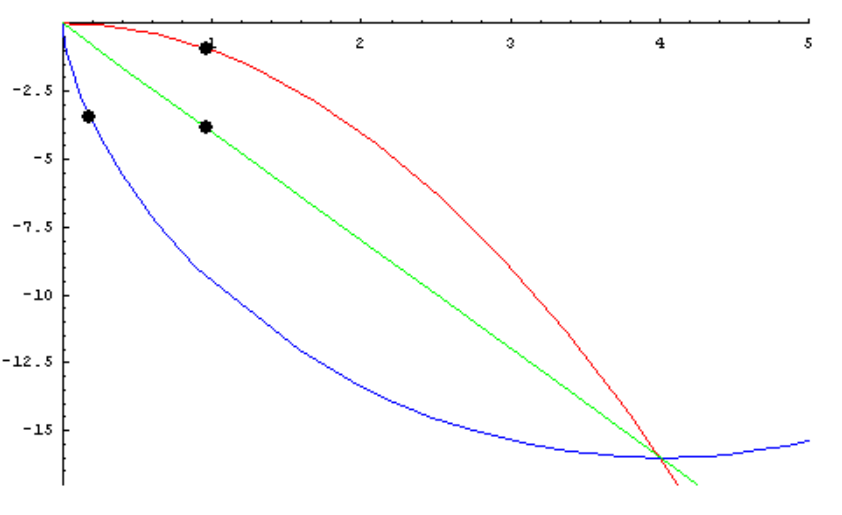
\includegraphics[width=10cm,keepaspectratio]{bra}

낙하 시간은 $\int^{y=h}_{y=0} \sqrt{\frac{1+(x^{\prime}(y))^2}{y}} dy$이다. 이 때, 적당한 상수 a에 대해서 $x=a(\theta-sin (\theta))$, $y = a(1-cos(\theta))$가 되어 사이클로이드가 된다. 
\end{frame}

\end{document}


